\documentclass{article}
\usepackage{graphicx} % Required for inserting images
\usepackage{kotex}
\usepackage{subfigure}
\usepackage{caption}

\title{프로그래밍 언어 HW5}
\author{B811079 방병훈}
\date{20230602}

\begin{document}
\maketitle
\section{Prolog에 대한 간단한 소개}
Prolog는 논리형 프로그래밍 언어로, 논리적 추론과 규칙 기반 프로그래밍을 기반으로 합니다.
1973년 프랑스의 알랭 코메르가가 개발한 언어로 오브젝트와 오브젝트 간의 관계에 관한 문제를 해결하기 위해 사용하고, 주로 인공지능, 전문 시스템, 자연 언어 처리 등 다양한 분야에서 활용됩니다. Prolog의 특징은 symbolic programming, declarative programming, logic programming으로 설명할 수 있습니다. 우선 symbolic programming이란, prolog가 수치연산 측면에서 취약하고 언어적인 지원이 협소하지만, 심볼 연산 관련 연구에서는 다른 언어로는 직관적이지 않은 코드가 prolog에서는 직관적으로 표현된다는 점입니다. 두번째로 declarative programming이란, 절차적 언어와 달리 선언적 패러다임으로 같은 문제에 대해서 다른 문제 해결방법을 강제한다는 것입니다. 마지막으로 logic programming은 논리를 프로그래밍 언어로 표현한다는 뜻입니다.
\section{Prolog의 문법}
\subsection{기본자료형}
{\bf 기본 자료형}\\
Prolog의 기본 자료형에는 아톰, 변수, 숫자, 리스트가 있습니다. 아톰은 데이터, 상수등으로 문자, 숫자, 언더바, ' 로 구성된 데이터입니다. 변수는 다른 언어와 다르게 저장공간을 의미하는게 아니라 관계를 표현하기위해 존재합니다. 변수는 무조건 첫 글자가 대문자나 \_ 밑줄로 시작해야합니다. 또한, 특수변수도 존재하는데 특수변수는 \_ 로 표현하고 어떠한 값이 와도 된다는 것을 뜻입니다. 숫자는 말그대로 숫자입니다. 마지막으로 리스트는 아톰, 변수, 숫자가 모여서 만들어진 데이터 형으로 대괄호[]로 표현됩니다. [1,two,'hi',B]가 리스트의 예 입니다. 또한, 리스트안에 리스트가 들어갈 수 있습니다. \\
\subsection{요소}
Prolog에는 세 가지 요소가 존재합니다. 사실, 규칙, 질문입니다.\\
{\bf 사실}\\
사실은 어떤 사실이나 정보를 true로 정의하는 것입니다. 예를 들어 male(brian).이면 brian은 male이라는 사실을 true로 정의한 것입니다. 관계와 객체의 이름은 소문자로 시작하고 관계의 이름을 먼저 쓰고, 객체들은 괄호 안에 쉼표로 구분합니다.
사실은 항상 . 으로 끝납니다. \\
{\bf 규칙}\\
규칙은 다른 사실로부터 또 다른 사실을 추론 가능하게 합니다. 형식은 Head :- Body로 해석하는 방법은 'Body가 true이면 Head도 true다' 입니다. Body에는 사실과 규칙이 여러개 들어갈 수 있습니다. Body부분의 ,는 논리 and의 의미이고 ;는 논리 or의 의미입니다. \\
{\bf 질문}\\
질문은 사실들을 저장한 후에 그에 대한 질문을 제기하는 것입니다. 질문은 사실과 유사하지만 그 앞에 특수기호 ?-가 붙어서 질문을 하면 그에 대한 결과가 나옵니다. \\
\subsection{디버깅}
{\bf Trace}\\
Prolog에서는 trace라는 기능을 통해서 디버깅을 지원합니다. trace는 질의 시에 질의 과정을 추적하는 역할을 하고 이를 통해서 내부적으로 어떤 과정에 의해서 코드가 실행되는지 이해할 수 있습니다. 특히, 재귀적인 호출 관계를 이해하는데 도움이 됩니다. trace. 이라는 명령어를 통해 trace 모드로 진입할 수 있고 nodebug. 명령어를 통해 trace 모드에서 탈출할 수 있습니다. trace 모드를 사용하게 되면 아톰의 자리에 숫자들이 나오는데 이는 임시 변수이고 엔터를 치면 나오는 creep은 엔터를 치면 나오는 결과입니다. 추가적으로 출력되는 명령어들을 살펴보면 call은 질의의 답을 찾기 위해 시도했다는 뜻이고, Exit은 질의에 대한 답을 구했다는 뜻이고, Redo는 질의의 답을 찾기위해 재시도했다는 뜻이고, Fail은 답을 찾기 실패했다는 뜻입니다.
\subsection{논리연산자}
Prolog의 논리연산자는 다른 언어와는 크게 다릅니다. 다른 언어들은 통상적으로 공유하는 관례가 있지만 prolog는 다릅니다. 
\begin{verbatim}
\+는 not, =\= 는 !=를 의미합니다. =:=는 ==, ,는 and , ;는 or, if(A==true) B 라는 코드는 A->B 즉, A이면 B이다로 해석해야합니다.
\end{verbatim}
논리연산자는 아니지만 명령어를 살펴보면 !는 cut으로 원치 않는 역추적을 방지하고, 불필요한 계산을 방지합니다. is는 =의 역할로 A is 1+2 이면 A = 3. 과 같은 말입니다. write는 화면에 문자열을 출려하기 위해서 사용합니다. nl은 newline을 의미합니다.

\section{코드}
\begin{figure}[h]
    \centering
    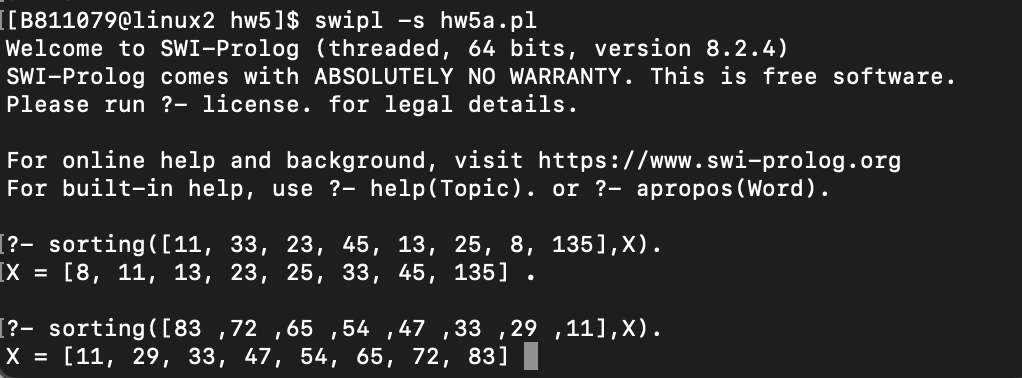
\includegraphics[width = 10cm,height = 6cm]{hw5a_run.png}
    \caption{hw5a 실행결과}
    \label{fig:fig1}
\end{figure}
\subsection{hw5a 코드}
\begin{verbatim}
% insert(X, List, Result)는 정렬된 리스트(List)에 원소(X)를 삽입해서 결과(Result)를 반환합니다.
insert(X, [], [X]). % 1. 빈 리스트에 원소를 삽입하면 그 원소만을 갖는 리스트를 반환합니다.
insert(X, [Y|Rest], [X,Y|Rest]) :- X =< Y. % 2. X<=Y이면 X를 Y 앞에 삽입합니다.
insert(X, [Y|Rest], [Y|Result]) :- X > Y, insert(X, Rest, Result). % 3. X>Y이면 Y를 결과 리스트에 유지한 채로 X를 재귀적으로 삽입합니다.

% sorting(List, Sortedlist)는 주어진 리스트(List)를 정렬하여 결과(Sortedlist)를 반환합니다.
sorting([], []). % 빈 리스트는 이미 정렬되어 있으므로 빈 리스트를 반환합니다.
sorting([X|Rest], Sortedlist) :- sorting(Rest, Psortedlist), insert(X, Psortedlist, Sortedlist). 
% 리스트를 재귀적으로 정렬한 후, 그 결과에 현재 원소 X를 삽입하여 전체 리스트를 정렬합니다.

%TC1 : [11, 33, 23, 45, 13, 25, 8, 135]
%TC2 : [83 ,72 ,65 ,54 ,47 ,33 ,29 ,11]
\end{verbatim}
Trace 결과
\begin{verbatim}
[trace]  ?- sorting([3,2,1],X).
   Call: (10) sorting([3, 2, 1], _9506) ? creep
   Call: (11) sorting([2, 1], _9962) ? creep
   Call: (12) sorting([1], _10006) ? creep
   Call: (13) sorting([], _10050) ? creep
   Exit: (13) sorting([], []) ? creep
   Call: (13) insert(1, [], _10140) ? creep
   Exit: (13) insert(1, [], [1]) ? creep
   Exit: (12) sorting([1], [1]) ? creep
   Call: (12) insert(2, [1], _10278) ? creep
   Call: (13) 2=<1 ? creep
   Fail: (13) 2=<1 ? creep
   Redo: (12) insert(2, [1], _10422) ? creep
   Call: (13) 2>1 ? creep
   Exit: (13) 2>1 ? creep
   Call: (13) insert(2, [], _10412) ? creep
   Exit: (13) insert(2, [], [2]) ? creep
   Exit: (12) insert(2, [1], [1, 2]) ? creep
   Exit: (11) sorting([2, 1], [1, 2]) ? creep
   Call: (11) insert(3, [1, 2], _9506) ? creep
   Call: (12) 3=<1 ? creep
   Fail: (12) 3=<1 ? creep
   Redo: (11) insert(3, [1, 2], _9506) ? creep
   Call: (12) 3>1 ? creep
   Exit: (12) 3>1 ? creep
   Call: (12) insert(3, [2], _10876) ? creep
   Call: (13) 3=<2 ? creep
   Fail: (13) 3=<2 ? creep
   Redo: (12) insert(3, [2], _10876) ? creep
   Call: (13) 3>2 ? creep
   Exit: (13) 3>2 ? creep
   Call: (13) insert(3, [], _11158) ? creep
   Exit: (13) insert(3, [], [3]) ? creep
   Exit: (12) insert(3, [2], [2, 3]) ? creep
   Exit: (11) insert(3, [1, 2], [1, 2, 3]) ? creep
   Exit: (10) sorting([3, 2, 1], [1, 2, 3]) ? creep
X = [1, 2, 3] .
\end{verbatim}
\begin{figure}[h]
    \centering
    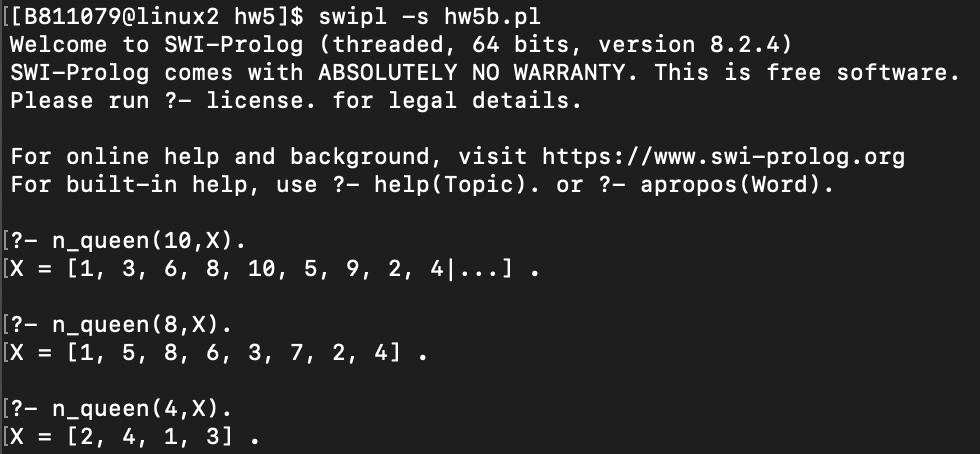
\includegraphics[width = 10cm,height = 6cm]{hw5b_run.png}
    \caption{hw5b 실행 결과}
    \label{fig:fig1}
\end{figure}
\subsection{hw5a 코드 작동 방식}
코드는 크게 두가지 부분으로 나뉘어있습니다. 정렬된 리스트에 원소를 삽입하는 insert부분과 요소를 정렬하는 sorting 부분입니다. insert 규칙은 크게 3부분으로 나뉘어있습니다. 우선 insert의 첫 규칙에 경우 빈 리스트에 대한 규칙 부분입니다. 빈 리스트에 원소를 삽입하면 그 원소만 갖는 리스트를 반환합니다. 두번째 규칙의 경우 기존의 리스트는 정렬이 되어있는데 기존의 리스트와 새로 추가하는 원소 X를 비교를 해야하는데 기존의 리스트는 정렬이 되어있으므로 맨왼쪽 원소인 Y와 비교해서 X가 더 작으면 왼쪽에 추가합니다. 그렇지 않은 경우에 대해서 insert의 세번째 규칙이 처리합니다. 만약 X가 Y보다 크면 X < Y일 때까지 재귀적으로 insert 규칙을 사용해서 삽입합니다. sorting의 경우 첫번째 규칙은 빈 리스트에 대한 규칙입니다. 빈 리스트에 대해서는 처리가 불필요하므로 빈리스트를 반환합니다. 두 번째 규칙의 경우는 [X|Rest]가 주어진 경우입니다. 리스트를 재귀적으로 정렬해서 Psortedlist에 저장하고 insert의 3번째 규칙을 활용해서 X를 Psortedlist에 삽입해서 Sortedlist를 구합니다. Rest는 리스트에서 X를 제외한 리스트입니다. sorting(Rest,Psortedlist)는 Rest를 재귀적으로 정렬한 결과인 Psortedlist를 구합니다. insert(X, Psortedlist, Sortedlist)는 X를 Psortedlist에 삽입하여 Sortedlist를 얻습니다. 

\subsection{Trace 분석}
처음에 sorting([3,2,1],X)를 입력하면 sorting의 두번째 규칙이 호출됩니다. 오른쪽의 숫자는 입력된 리스트 [3,2,1]을 저장할 임시 변수입니다. 이후에 재귀적으로 다시 sorting의 두번째 규칙이 호출돼서 첫번째 원소 3을 제외한 [2,1]가 임시변수에 저장됩니다. 다시 sorting의 두번째 규칙이 호출돼서 두번째 원소 2를 제외한 [1]을 임시변수에 저장합니다. 두번째 sorting 규칙이 호출됩니다. 그런데 이미 빈 리스트이므로 첫번째 규칙이 호출되고 빈 리스트 []에 마지막 원소 1을 삽입하고 임시변수에 저장합니다. 이를 sorting하면 당연히 리스트에 1밖에 없으므로 정렬을 해도 [1]입니다. 이후에 두번째 원소 2가 삽입되는데 insert의 3번째 규칙이 호출됩니다. trace를 확인하면 1과 2의 크기를 비교합니다. 이는 insert의 규칙적용을 위한 절차입니다. 이후 insert의 3번쨰 규칙을 활용해서 2를 1의 뒤에 삽입한 [1,2]가 임시변수에 저장된다. sorting([2,1],[1,2])에서 오른쪽을 보면 부분적으로 정렬이 된 리스트이다. 이후 insert 규칙을 호출한다. 3을 [1,2]의 원소들과 크기비교를 하고 3을 맨 뒤에 삽입하고 정렬을 마친다. X = [1,2,3]으로 결과가 출력된다.
\subsection{hw5b 코드}
\begin{verbatim}
% 체스판 위에 퀸을 배치하는 규칙 정의
% 퀸이 다른 퀸과 같은 행 또는 열에 있으면 안 됨
% 퀸이 다른 퀸의 대각선에 있으면 안 됨
% N행 1열부터 N행 N열까지 퀸을 배치하는 규칙 정의

n_queen(N, Queens) :- 
    range(1, N, Rows), % 1부터 N까지의 숫자 리스트를 생성해서 Rows에 저장합니다.
    permutation(Rows, Queens), % Rows의 순열을 생성하여 Queens에 저장합니다.
    safe(Queens). % Queens의 퀸들이 서로 공격할 수 없는 위치에 있는지 확인합니다.

% range(Start, End, List)는 Start에서 End까지의 숫자들을 리스트 List로 생성하는 규칙
range(Start, Start, [Start]).
range(Start, End, [Start|List]) :- 
    Start < End, 
    Start1 is Start + 1, 
    range(Start1, End, List).

% permutation은 가능한 모든 퀸의 배치를 생성하기 위해 사용됩니다.
permutation([], []).
permutation(List, [X|Perm]) :- 
    select(X, List, Rest), % List에서 X 선택하여 Rest에 저장합니다.
    permutation(Rest, Perm).

% safe(Queens)는 Queens의 퀸들이 서로 공격할 수 없는 위치에 있는지 확인합니다.
safe([]).   %빈 리스트이면 당연히 퀸들이 서로 공격할수 없습니다.
safe([Queen|Otherqueens]) :- 
    safe(Otherqueens), % Otherqueens에 있는 퀸들이 서로 공격할 수 없는지 확인합니다.
    check(Queen, Otherqueens, 1).%첫번째 열부터 검사 시작.

% check(Queen, Otherqueens, N)은 주어진 위치에 퀸을 배치할때 배치한 위치가 다른 퀸과 공격가능한지 파악합니다.
% Queen은 현재 검사중인 퀸의 행 번호입니다. Otherqueens는 이전에 배치된 퀸들의 위치를 나타내는 리스트입니다.
check(_, [], _). %이전에 배치된 퀸이 없을때는 검사할 필요가 없습니다.
check(Y, [Y1|Ylist], Xdist) :-  %Y는 현재 검사중인 퀸의 행번호 [Y1|Ylist]는 이전 배치된 퀸들의 행 번호를 저장하고있습니다. 
                                % Xdist는 현재 검사중인 퀸과 이전 퀸들의 열 번호 차이를 의미합니다.
    Y1 - Y =\= Xdist, % 오른쪽 대각선에 겹치는 퀸을 확인합니다.
    Y - Y1 =\= Xdist, % 왼쪽 대각선에 겹치는 퀸을 확인합니다.
    Dist1 is Xdist + 1, %다음 열 번호 차이를 계산합니다.
    check(Y, Ylist, Dist1). %이전 퀸과 충돌하는지 재귀적으로 검사.

\end{verbatim}
\subsection{Trace 결과}
\begin{verbatim}
    [trace]  ?- n_queen(4,X).
   Call: (10) n_queen(4, _6946) ? creep
   Call: (11) range(1, 4, _7384) ? creep
   Call: (12) 1<4 ? creep
   Exit: (12) 1<4 ? creep
   Call: (12) _7524 is 1+1 ? creep
   Exit: (12) 2 is 1+1 ? creep
   Call: (12) range(2, 4, _7374) ? creep
   Call: (13) 2<4 ? creep
   Exit: (13) 2<4 ? creep
   Call: (13) _7756 is 2+1 ? creep
   Exit: (13) 3 is 2+1 ? creep
   Call: (13) range(3, 4, _7606) ? creep
   Call: (14) 3<4 ? creep
   Exit: (14) 3<4 ? creep
   Call: (14) _7988 is 3+1 ? creep
   Exit: (14) 4 is 3+1 ? creep
   Call: (14) range(4, 4, _7838) ? creep
   Exit: (14) range(4, 4, [4]) ? creep
   Exit: (13) range(3, 4, [3, 4]) ? creep
   Exit: (12) range(2, 4, [2, 3, 4]) ? creep
   Exit: (11) range(1, 4, [1, 2, 3, 4]) ? creep
   Call: (11) permutation([1, 2, 3, 4], _6946) ? creep
   Call: (12) lists:select(_8294, [1, 2, 3, 4], _8526) ? creep
   Exit: (12) lists:select(1, [1, 2, 3, 4], [2, 3, 4]) ? creep
   Call: (12) permutation([2, 3, 4], _8296) ? creep
   Call: (13) lists:select(_8602, [2, 3, 4], _8664) ? creep
   Exit: (13) lists:select(2, [2, 3, 4], [3, 4]) ? creep
   Call: (13) permutation([3, 4], _8604) ? creep
   Call: (14) lists:select(_8740, [3, 4], _8802) ? creep
   Exit: (14) lists:select(3, [3, 4], [4]) ? creep
   Call: (14) permutation([4], _8742) ? creep
   Call: (15) lists:select(_8878, [4], _8940) ? creep
   Exit: (15) lists:select(4, [4], []) ? creep
   Call: (15) permutation([], _8880) ? creep
   Exit: (15) permutation([], []) ? creep
   Exit: (14) permutation([4], [4]) ? creep
   Exit: (13) permutation([3, 4], [3, 4]) ? creep
   Exit: (12) permutation([2, 3, 4], [2, 3, 4]) ? creep
   Exit: (11) permutation([1, 2, 3, 4], [1, 2, 3, 4]) ? creep
   Call: (11) safe([1, 2, 3, 4]) ? creep
   Call: (12) safe([2, 3, 4]) ? creep
   Call: (13) safe([3, 4]) ? creep
   Call: (14) safe([4]) ? creep
   Call: (15) safe([]) ? creep
   Exit: (15) safe([]) ? creep
   Call: (15) check(4, [], 1) ? creep
   Exit: (15) check(4, [], 1) ? creep
   Exit: (14) safe([4]) ? creep
   Call: (14) check(3, [4], 1) ? creep
   Call: (15) 4-3=\=1 ? creep
   Fail: (15) 4-3=\=1 ? creep
   Fail: (14) check(3, [4], 1) ? creep
   Redo: (15) check(4, [], 1) ? creep
   Fail: (15) check(4, [], 1) ? creep
   Fail: (14) safe([4]) ? creep
   Fail: (13) safe([3, 4]) ? creep
   Fail: (12) safe([2, 3, 4]) ? creep
   Fail: (11) safe([1, 2, 3, 4]) ? creep
   Redo: (15) permutation([], _8880) ? creep
   Call: (16) lists:select(_10122, [], _10184) ? creep
   Fail: (16) lists:select(_10122, [], _10228) ? creep
   Fail: (15) permutation([], _8880) ? creep
   Fail: (14) permutation([4], _8742) ? creep
   Redo: (14) lists:select(_8740, [3, 4], _10360) ? creep
   Exit: (14) lists:select(4, [3, 4], [3]) ? creep
   Call: (14) permutation([3], _8742) ? creep
   Call: (15) lists:select(_10442, [3], _10504) ? creep
   Exit: (15) lists:select(3, [3], []) ? creep
   Call: (15) permutation([], _10444) ? creep
   Exit: (15) permutation([], []) ? creep
   Exit: (14) permutation([3], [3]) ? creep
   Exit: (13) permutation([3, 4], [4, 3]) ? creep
   Exit: (12) permutation([2, 3, 4], [2, 4, 3]) ? creep
   Exit: (11) permutation([1, 2, 3, 4], [1, 2, 4, 3]) ? creep
   Call: (11) safe([1, 2, 4, 3]) ? creep
   Call: (12) safe([2, 4, 3]) ? creep
   Call: (13) safe([4, 3]) ? creep
   Call: (14) safe([3]) ? creep
   Call: (15) safe([]) ? creep
   Exit: (15) safe([]) ? creep
   Call: (15) check(3, [], 1) ? creep
   Exit: (15) check(3, [], 1) ? creep
   Exit: (14) safe([3]) ? creep
   Call: (14) check(4, [3], 1) ? creep
   Call: (15) 3-4=\=1 ? creep
   Exit: (15) 3-4=\=1 ? creep
   Call: (15) 4-3=\=1 ? creep
   Fail: (15) 4-3=\=1 ? creep
   Fail: (14) check(4, [3], 1) ? creep
   Redo: (15) check(3, [], 1) ? creep
   Fail: (15) check(3, [], 1) ? creep
   Fail: (14) safe([3]) ? creep
   Fail: (13) safe([4, 3]) ? creep
   Fail: (12) safe([2, 4, 3]) ? creep
   Fail: (11) safe([1, 2, 4, 3]) ? creep
   Redo: (15) permutation([], _10444) ? creep
   Call: (16) lists:select(_11780, [], _11842) ? creep
   Fail: (16) lists:select(_11780, [], _11886) ? creep
   Fail: (15) permutation([], _10444) ? creep
   Fail: (14) permutation([3], _8742) ? creep
   Fail: (13) permutation([3, 4], _8604) ? creep
   Redo: (13) lists:select(_8602, [2, 3, 4], _12062) ? creep
   Exit: (13) lists:select(3, [2, 3, 4], [2, 4]) ? creep
   Call: (13) permutation([2, 4], _8604) ? creep
   Call: (14) lists:select(_12144, [2, 4], _12206) ? creep
   Exit: (14) lists:select(2, [2, 4], [4]) ? creep
   Call: (14) permutation([4], _12146) ? creep
   Call: (15) lists:select(_12282, [4], _12344) ? creep
   Exit: (15) lists:select(4, [4], []) ? creep
   Call: (15) permutation([], _12284) ? creep
   Exit: (15) permutation([], []) ? creep
   Exit: (14) permutation([4], [4]) ? creep
   Exit: (13) permutation([2, 4], [2, 4]) ? creep
   Exit: (12) permutation([2, 3, 4], [3, 2, 4]) ? creep
   Exit: (11) permutation([1, 2, 3, 4], [1, 3, 2, 4]) ? creep
   Call: (11) safe([1, 3, 2, 4]) ? creep
   Call: (12) safe([3, 2, 4]) ? creep
   Call: (13) safe([2, 4]) ? creep
   Call: (14) safe([4]) ? creep
   Call: (15) safe([]) ? creep
   Exit: (15) safe([]) ? creep
   Call: (15) check(4, [], 1) ? creep
   Exit: (15) check(4, [], 1) ? creep
   Exit: (14) safe([4]) ? creep
   Call: (14) check(2, [4], 1) ? creep
   Call: (15) 4-2=\=1 ? creep
   Exit: (15) 4-2=\=1 ? creep
   Call: (15) 2-4=\=1 ? creep
   Exit: (15) 2-4=\=1 ? creep
   Call: (15) _13326 is 1+1 ? creep
   Exit: (15) 2 is 1+1 ? creep
   Call: (15) check(2, [], 2) ? creep
   Exit: (15) check(2, [], 2) ? creep
   Exit: (14) check(2, [4], 1) ? creep
   Exit: (13) safe([2, 4]) ? creep
   Call: (13) check(3, [2, 4], 1) ? creep
   Call: (14) 2-3=\=1 ? creep
   Exit: (14) 2-3=\=1 ? creep
   Call: (14) 3-2=\=1 ? creep
   Fail: (14) 3-2=\=1 ? creep
   Fail: (13) check(3, [2, 4], 1) ? creep
   Redo: (15) check(2, [], 2) ? creep
   Fail: (15) check(2, [], 2) ? creep
   Fail: (14) check(2, [4], 1) ? creep
   Redo: (15) check(4, [], 1) ? creep
   Fail: (15) check(4, [], 1) ? creep
   Fail: (14) safe([4]) ? creep
   Fail: (13) safe([2, 4]) ? creep
   Fail: (12) safe([3, 2, 4]) ? creep
   Fail: (11) safe([1, 3, 2, 4]) ? creep
   Redo: (15) permutation([], _12284) ? creep
   Call: (16) lists:select(_14254, [], _14316) ? creep
   Fail: (16) lists:select(_14254, [], _14360) ? creep
   Fail: (15) permutation([], _12284) ? creep
   Fail: (14) permutation([4], _12146) ? creep
   Redo: (14) lists:select(_12144, [2, 4], _14492) ? creep
   Exit: (14) lists:select(4, [2, 4], [2]) ? creep
   Call: (14) permutation([2], _12146) ? creep
   Call: (15) lists:select(_14574, [2], _14636) ? creep
   Exit: (15) lists:select(2, [2], []) ? creep
   Call: (15) permutation([], _14576) ? creep
   Exit: (15) permutation([], []) ? creep
   Exit: (14) permutation([2], [2]) ? creep
   Exit: (13) permutation([2, 4], [4, 2]) ? creep
   Exit: (12) permutation([2, 3, 4], [3, 4, 2]) ? creep
   Exit: (11) permutation([1, 2, 3, 4], [1, 3, 4, 2]) ? creep
   Call: (11) safe([1, 3, 4, 2]) ? creep
   Call: (12) safe([3, 4, 2]) ? creep
   Call: (13) safe([4, 2]) ? creep
   Call: (14) safe([2]) ? creep
   Call: (15) safe([]) ? creep
   Exit: (15) safe([]) ? creep
   Call: (15) check(2, [], 1) ? creep
   Exit: (15) check(2, [], 1) ? creep
   Exit: (14) safe([2]) ? creep
   Call: (14) check(4, [2], 1) ? creep
   Call: (15) 2-4=\=1 ? creep
   Exit: (15) 2-4=\=1 ? creep
   Call: (15) 4-2=\=1 ? creep
   Exit: (15) 4-2=\=1 ? creep
   Call: (15) _15618 is 1+1 ? creep
   Exit: (15) 2 is 1+1 ? creep
   Call: (15) check(4, [], 2) ? creep
   Exit: (15) check(4, [], 2) ? creep
   Exit: (14) check(4, [2], 1) ? creep
   Exit: (13) safe([4, 2]) ? creep
   Call: (13) check(3, [4, 2], 1) ? creep
   Call: (14) 4-3=\=1 ? creep
   Fail: (14) 4-3=\=1 ? creep
   Fail: (13) check(3, [4, 2], 1) ? creep
   Redo: (15) check(4, [], 2) ? creep
   Fail: (15) check(4, [], 2) ? creep
   Fail: (14) check(4, [2], 1) ? creep
   Redo: (15) check(2, [], 1) ? creep
   Fail: (15) check(2, [], 1) ? creep
   Fail: (14) safe([2]) ? creep
   Fail: (13) safe([4, 2]) ? creep
   Fail: (12) safe([3, 4, 2]) ? creep
   Fail: (11) safe([1, 3, 4, 2]) ? creep
   Redo: (15) permutation([], _14576) ? creep
   Call: (16) lists:select(_16452, [], _16514) ? creep
   Fail: (16) lists:select(_16452, [], _16558) ? creep
   Fail: (15) permutation([], _14576) ? creep
   Fail: (14) permutation([2], _12146) ? creep
   Fail: (13) permutation([2, 4], _8604) ? creep
   Redo: (13) lists:select(_8602, [2, 3, 4], [2|_12052]) ? creep
   Exit: (13) lists:select(4, [2, 3, 4], [2, 3]) ? creep
   Call: (13) permutation([2, 3], _8604) ? creep
   Call: (14) lists:select(_16816, [2, 3], _16878) ? creep
   Exit: (14) lists:select(2, [2, 3], [3]) ? creep
   Call: (14) permutation([3], _16818) ? creep
   Call: (15) lists:select(_16954, [3], _17016) ? creep
   Exit: (15) lists:select(3, [3], []) ? creep
   Call: (15) permutation([], _16956) ? creep
   Exit: (15) permutation([], []) ? creep
   Exit: (14) permutation([3], [3]) ? creep
   Exit: (13) permutation([2, 3], [2, 3]) ? creep
   Exit: (12) permutation([2, 3, 4], [4, 2, 3]) ? creep
   Exit: (11) permutation([1, 2, 3, 4], [1, 4, 2, 3]) ? creep
   Call: (11) safe([1, 4, 2, 3]) ? creep
   Call: (12) safe([4, 2, 3]) ? creep
   Call: (13) safe([2, 3]) ? creep
   Call: (14) safe([3]) ? creep
   Call: (15) safe([]) ? creep
   Exit: (15) safe([]) ? creep
   Call: (15) check(3, [], 1) ? creep
   Exit: (15) check(3, [], 1) ? creep
   Exit: (14) safe([3]) ? creep
   Call: (14) check(2, [3], 1) ? creep
   Call: (15) 3-2=\=1 ? creep
   Fail: (15) 3-2=\=1 ? creep
   Fail: (14) check(2, [3], 1) ? creep
   Redo: (15) check(3, [], 1) ? creep
   Fail: (15) check(3, [], 1) ? creep
   Fail: (14) safe([3]) ? creep
   Fail: (13) safe([2, 3]) ? creep
   Fail: (12) safe([4, 2, 3]) ? creep
   Fail: (11) safe([1, 4, 2, 3]) ? creep
   Redo: (15) permutation([], _16956) ? creep
   Call: (16) lists:select(_18198, [], _18260) ? creep
   Fail: (16) lists:select(_18198, [], _18304) ? creep
   Fail: (15) permutation([], _16956) ? creep
   Fail: (14) permutation([3], _16818) ? creep
   Redo: (14) lists:select(_16816, [2, 3], _18436) ? creep
   Exit: (14) lists:select(3, [2, 3], [2]) ? creep
   Call: (14) permutation([2], _16818) ? creep
   Call: (15) lists:select(_18518, [2], _18580) ? creep
   Exit: (15) lists:select(2, [2], []) ? creep
   Call: (15) permutation([], _18520) ? creep
   Exit: (15) permutation([], []) ? creep
   Exit: (14) permutation([2], [2]) ? creep
   Exit: (13) permutation([2, 3], [3, 2]) ? creep
   Exit: (12) permutation([2, 3, 4], [4, 3, 2]) ? creep
   Exit: (11) permutation([1, 2, 3, 4], [1, 4, 3, 2]) ? creep
   Call: (11) safe([1, 4, 3, 2]) ? creep
   Call: (12) safe([4, 3, 2]) ? creep
   Call: (13) safe([3, 2]) ? creep
   Call: (14) safe([2]) ? creep
   Call: (15) safe([]) ? creep
   Exit: (15) safe([]) ? creep
   Call: (15) check(2, [], 1) ? creep
   Exit: (15) check(2, [], 1) ? creep
   Exit: (14) safe([2]) ? creep
   Call: (14) check(3, [2], 1) ? creep
   Call: (15) 2-3=\=1 ? creep
   Exit: (15) 2-3=\=1 ? creep
   Call: (15) 3-2=\=1 ? creep
   Fail: (15) 3-2=\=1 ? creep
   Fail: (14) check(3, [2], 1) ? creep
   Redo: (15) check(2, [], 1) ? creep
   Fail: (15) check(2, [], 1) ? creep
   Fail: (14) safe([2]) ? creep
   Fail: (13) safe([3, 2]) ? creep
   Fail: (12) safe([4, 3, 2]) ? creep
   Fail: (11) safe([1, 4, 3, 2]) ? creep
   Redo: (15) permutation([], _18520) ? creep
   Call: (16) lists:select(_19856, [], _19918) ? creep
   Fail: (16) lists:select(_19856, [], _19962) ? creep
   Fail: (15) permutation([], _18520) ? creep
   Fail: (14) permutation([2], _16818) ? creep
   Fail: (13) permutation([2, 3], _8604) ? creep
   Fail: (12) permutation([2, 3, 4], _8296) ? creep
   Redo: (12) lists:select(_8294, [1, 2, 3, 4], _20182) ? creep
   Exit: (12) lists:select(2, [1, 2, 3, 4], [1, 3, 4]) ? creep
   Call: (12) permutation([1, 3, 4], _8296) ? creep
   Call: (13) lists:select(_20264, [1, 3, 4], _20326) ? creep
   Exit: (13) lists:select(1, [1, 3, 4], [3, 4]) ? creep
   Call: (13) permutation([3, 4], _20266) ? creep
   Call: (14) lists:select(_20402, [3, 4], _20464) ? creep
   Exit: (14) lists:select(3, [3, 4], [4]) ? creep
   Call: (14) permutation([4], _20404) ? creep
   Call: (15) lists:select(_20540, [4], _20602) ? creep
   Exit: (15) lists:select(4, [4], []) ? creep
   Call: (15) permutation([], _20542) ? creep
   Exit: (15) permutation([], []) ? creep
   Exit: (14) permutation([4], [4])


 ? creep
   Exit: (13) permutation([3, 4], [3, 4]) ? creep
   Exit: (12) permutation([1, 3, 4], [1, 3, 4]) ? creep
   Exit: (11) permutation([1, 2, 3, 4], [2, 1, 3, 4]) ? creep
   Call: (11) safe([2, 1, 3, 4]) ? creep
   Call: (12) safe([1, 3, 4]) ? creep
   Call: (13) safe([3, 4]) ? creep
   Call: (14) safe([4]) ? creep
   Call: (15) safe([]) ? creep
   Exit: (15) safe([]) ? creep
   Call: (15) check(4, [], 1) ? creep
   Exit: (15) check(4, [], 1) ? creep
   Exit: (14) safe([4]) ? creep
   Call: (14) check(3, [4], 1) ? creep
   Call: (15) 4-3=\=1 ? creep
   Fail: (15) 4-3=\=1 ? creep
   Fail: (14) check(3, [4], 1) ? creep
   Redo: (15) check(4, [], 1) ? creep
   Fail: (15) check(4, [], 1) ? creep
   Fail: (14) safe([4]) ? creep
   Fail: (13) safe([3, 4]) ? creep
   Fail: (12) safe([1, 3, 4]) ? creep
   Fail: (11) safe([2, 1, 3, 4]) ? creep
   Redo: (15) permutation([], _20542) ? creep
   Call: (16) lists:select(_21784, [], _21846) ? creep
   Fail: (16) lists:select(_21784, [], _21890) ? creep
   Fail: (15) permutation([], _20542) ? creep
   Fail: (14) permutation([4], _20404) ? creep
   Redo: (14) lists:select(_20402, [3, 4], _22022) ? creep
   Exit: (14) lists:select(4, [3, 4], [3]) ? creep
   Call: (14) permutation([3], _20404) ? creep
   Call: (15) lists:select(_22104, [3], _22166) ? creep
   Exit: (15) lists:select(3, [3], []) ? creep
   Call: (15) permutation([], _22106) ? creep
   Exit: (15) permutation([], []) ? creep
   Exit: (14) permutation([3], [3]) ? creep
   Exit: (13) permutation([3, 4], [4, 3]) ? creep
   Exit: (12) permutation([1, 3, 4], [1, 4, 3]) ? creep
   Exit: (11) permutation([1, 2, 3, 4], [2, 1, 4, 3]) ? creep
   Call: (11) safe([2, 1, 4, 3]) ? creep
   Call: (12) safe([1, 4, 3]) ? creep
   Call: (13) safe([4, 3]) ? creep
   Call: (14) safe([3]) ? creep
   Call: (15) safe([]) ? creep
   Exit: (15) safe([]) ? creep
   Call: (15) check(3, [], 1) ? creep
   Exit: (15) check(3, [], 1) ? creep
   Exit: (14) safe([3]) ? creep
   Call: (14) check(4, [3], 1) ? creep
   Call: (15) 3-4=\=1 ? creep
   Exit: (15) 3-4=\=1 ? creep
   Call: (15) 4-3=\=1 ? creep
   Fail: (15) 4-3=\=1 ? creep
   Fail: (14) check(4, [3], 1) ? creep
   Redo: (15) check(3, [], 1) ? creep
   Fail: (15) check(3, [], 1) ? creep
   Fail: (14) safe([3]) ? creep
   Fail: (13) safe([4, 3]) ? creep
   Fail: (12) safe([1, 4, 3]) ? creep
   Fail: (11) safe([2, 1, 4, 3]) ? creep
   Redo: (15) permutation([], _22106) ? creep
   Call: (16) lists:select(_23442, [], _23504) ? creep
   Fail: (16) lists:select(_23442, [], _23548) ? creep
   Fail: (15) permutation([], _22106) ? creep
   Fail: (14) permutation([3], _20404) ? creep
   Fail: (13) permutation([3, 4], _20266) ? creep
   Redo: (13) lists:select(_20264, [1, 3, 4], _23724) ? creep
   Exit: (13) lists:select(3, [1, 3, 4], [1, 4]) ? creep
   Call: (13) permutation([1, 4], _20266) ? creep
   Call: (14) lists:select(_23806, [1, 4], _23868) ? creep
   Exit: (14) lists:select(1, [1, 4], [4]) ? creep
   Call: (14) permutation([4], _23808) ? creep
   Call: (15) lists:select(_23944, [4], _24006) ? creep
   Exit: (15) lists:select(4, [4], []) ? creep
   Call: (15) permutation([], _23946) ? creep
   Exit: (15) permutation([], []) ? creep
   Exit: (14) permutation([4], [4]) ? creep
   Exit: (13) permutation([1, 4], [1, 4]) ? creep
   Exit: (12) permutation([1, 3, 4], [3, 1, 4]) ? creep
   Exit: (11) permutation([1, 2, 3, 4], [2, 3, 1, 4]) ? creep
   Call: (11) safe([2, 3, 1, 4]) ? creep
   Call: (12) safe([3, 1, 4]) ? creep
   Call: (13) safe([1, 4]) ? creep
   Call: (14) safe([4]) ? creep
   Call: (15) safe([]) ? creep
   Exit: (15) safe([]) ? creep
   Call: (15) check(4, [], 1) ? creep
   Exit: (15) check(4, [], 1) ? creep
   Exit: (14) safe([4]) ? creep
   Call: (14) check(1, [4], 1) ? creep
   Call: (15) 4-1=\=1 ? creep
   Exit: (15) 4-1=\=1 ? creep
   Call: (15) 1-4=\=1 ? creep
   Exit: (15) 1-4=\=1 ? creep
   Call: (15) _24988 is 1+1 ? creep
   Exit: (15) 2 is 1+1 ? creep
   Call: (15) check(1, [], 2) ? creep
   Exit: (15) check(1, [], 2) ? creep
   Exit: (14) check(1, [4], 1) ? creep
   Exit: (13) safe([1, 4]) ? creep
   Call: (13) check(3, [1, 4], 1) ? creep
   Call: (14) 1-3=\=1 ? creep
   Exit: (14) 1-3=\=1 ? creep
   Call: (14) 3-1=\=1 ? creep
   Exit: (14) 3-1=\=1 ? creep
   Call: (14) _25490 is 1+1 ? creep
   Exit: (14) 2 is 1+1 ? creep
   Call: (14) check(3, [4], 2) ? creep
   Call: (15) 4-3=\=2 ? creep
   Exit: (15) 4-3=\=2 ? creep
   Call: (15) 3-4=\=2 ? creep
   Exit: (15) 3-4=\=2 ? creep
   Call: (15) _25816 is 2+1 ? creep
   Exit: (15) 3 is 2+1 ? creep
   Call: (15) check(3, [], 3) ? creep
   Exit: (15) check(3, [], 3) ? creep
   Exit: (14) check(3, [4], 2) ? creep
   Exit: (13) check(3, [1, 4], 1) ? creep
   Exit: (12) safe([3, 1, 4]) ? creep
   Call: (12) check(2, [3, 1, 4], 1) ? creep
   Call: (13) 3-2=\=1 ? creep
   Fail: (13) 3-2=\=1 ? creep
   Fail: (12) check(2, [3, 1, 4], 1) ? creep
   Redo: (15) check(3, [], 3) ? creep
   Fail: (15) check(3, [], 3) ? creep
   Fail: (14) check(3, [4], 2) ? creep
   Fail: (13) check(3, [1, 4], 1) ? creep
   Redo: (15) check(1, [], 2) ? creep
   Fail: (15) check(1, [], 2) ? creep
   Fail: (14) check(1, [4], 1) ? creep
   Redo: (15) check(4, [], 1) ? creep
   Fail: (15) check(4, [], 1) ? creep
   Fail: (14) safe([4]) ? creep
   Fail: (13) safe([1, 4]) ? creep
   Fail: (12) safe([3, 1, 4]) ? creep
   Fail: (11) safe([2, 3, 1, 4]) ? creep
   Redo: (15) permutation([], _23946) ? creep
   Call: (16) lists:select(_26870, [], _26932) ? creep
   Fail: (16) lists:select(_26870, [], _26976) ? creep
   Fail: (15) permutation([], _23946) ? creep
   Fail: (14) permutation([4], _23808) ? creep
   Redo: (14) lists:select(_23806, [1, 4], _27108) ? creep
   Exit: (14) lists:select(4, [1, 4], [1]) ? creep
   Call: (14) permutation([1], _23808) ? creep
   Call: (15) lists:select(_27190, [1], _27252) ? creep
   Exit: (15) lists:select(1, [1], []) ? creep
   Call: (15) permutation([], _27192) ? creep
   Exit: (15) permutation([], []) ? creep
   Exit: (14) permutation([1], [1]) ? creep
   Exit: (13) permutation([1, 4], [4, 1]) ? creep
   Exit: (12) permutation([1, 3, 4], [3, 4, 1]) ? creep
   Exit: (11) permutation([1, 2, 3, 4], [2, 3, 4, 1]) ? creep
   Call: (11) safe([2, 3, 4, 1]) ? creep
   Call: (12) safe([3, 4, 1]) ? creep
   Call: (13) safe([4, 1]) ? creep
   Call: (14) safe([1]) ? creep
   Call: (15) safe([]) ? creep
   Exit: (15) safe([]) ? creep
   Call: (15) check(1, [], 1) ? creep
   Exit: (15) check(1, [], 1) ? creep
   Exit: (14) safe([1]) ? creep
   Call: (14) check(4, [1], 1) ? creep
   Call: (15) 1-4=\=1 ? creep
   Exit: (15) 1-4=\=1 ? creep
   Call: (15) 4-1=\=1 ? creep
   Exit: (15) 4-1=\=1 ? creep
   Call: (15) _28234 is 1+1 ? creep
   Exit: (15) 2 is 1+1 ? creep
   Call: (15) check(4, [], 2) ? creep
   Exit: (15) check(4, [], 2) ? creep
   Exit: (14) check(4, [1], 1) ? creep
   Exit: (13) safe([4, 1]) ? creep
   Call: (13) check(3, [4, 1], 1) ? creep
   Call: (14) 4-3=\=1 ? creep
   Fail: (14) 4-3=\=1 ? creep
   Fail: (13) check(3, [4, 1], 1) ? creep
   Redo: (15) check(4, [], 2) ? creep
   Fail: (15) check(4, [], 2) ? creep
   Fail: (14) check(4, [1], 1) ? creep
   Redo: (15) check(1, [], 1) ? creep
   Fail: (15) check(1, [], 1) ? creep
   Fail: (14) safe([1]) ? creep
   Fail: (13) safe([4, 1]) ? creep
   Fail: (12) safe([3, 4, 1]) ? creep
   Fail: (11) safe([2, 3, 4, 1]) ? creep
   Redo: (15) permutation([], _27192) ? creep
   Call: (16) lists:select(_29068, [], _29130) ? creep
   Fail: (16) lists:select(_29068, [], _29174) ? creep
   Fail: (15) permutation([], _27192) ? creep
   Fail: (14) permutation([1], _23808) ? creep
   Fail: (13) permutation([1, 4], _20266) ? creep
   Redo: (13) lists:select(_20264, [1, 3, 4], [1|_23714]) ? creep
   Exit: (13) lists:select(4, [1, 3, 4], [1, 3]) ? creep
   Call: (13) permutation([1, 3], _20266) ? creep
   Call: (14) lists:select(_29432, [1, 3], _29494) ? creep
   Exit: (14) lists:select(1, [1, 3], [3]) ? creep
   Call: (14) permutation([3], _29434) ? creep
   Call: (15) lists:select(_29570, [3], _29632) ? creep
   Exit: (15) lists:select(3, [3], []) ? creep
   Call: (15) permutation([], _29572) ? creep
   Exit: (15) permutation([], []) ? creep
   Exit: (14) permutation([3], [3]) ? creep
   Exit: (13) permutation([1, 3], [1, 3]) ? creep
   Exit: (12) permutation([1, 3, 4], [4, 1, 3]) ? creep
   Exit: (11) permutation([1, 2, 3, 4], [2, 4, 1, 3]) ? creep
   Call: (11) safe([2, 4, 1, 3]) ? creep
   Call: (12) safe([4, 1, 3]) ? creep
   Call: (13) safe([1, 3]) ? creep
   Call: (14) safe([3]) ? creep
   Call: (15) safe([]) ? creep
   Exit: (15) safe([]) ? creep
   Call: (15) check(3, [], 1) ? creep
   Exit: (15) check(3, [], 1) ? creep
   Exit: (14) safe([3]) ? creep
   Call: (14) check(1, [3], 1) ? creep
   Call: (15) 3-1=\=1 ? creep
   Exit: (15) 3-1=\=1 ? creep
   Call: (15) 1-3=\=1 ? creep
   Exit: (15) 1-3=\=1 ? creep
   Call: (15) _30614 is 1+1 ? creep
   Exit: (15) 2 is 1+1 ? creep
   Call: (15) check(1, [], 2) ? creep
   Exit: (15) check(1, [], 2) ? creep
   Exit: (14) check(1, [3], 1) ? creep
   Exit: (13) safe([1, 3]) ? creep
   Call: (13) check(4, [1, 3], 1) ? creep
   Call: (14) 1-4=\=1 ? creep
   Exit: (14) 1-4=\=1 ? creep
   Call: (14) 4-1=\=1 ? creep
   Exit: (14) 4-1=\=1 ? creep
   Call: (14) _31116 is 1+1 ? creep
   Exit: (14) 2 is 1+1 ? creep
   Call: (14) check(4, [3], 2) ? creep
   Call: (15) 3-4=\=2 ? creep
   Exit: (15) 3-4=\=2 ? creep
   Call: (15) 4-3=\=2 ? creep
   Exit: (15) 4-3=\=2 ? creep
   Call: (15) _31442 is 2+1 ? creep
   Exit: (15) 3 is 2+1 ? creep
   Call: (15) check(4, [], 3) ? creep
   Exit: (15) check(4, [], 3) ? creep
   Exit: (14) check(4, [3], 2) ? creep
   Exit: (13) check(4, [1, 3], 1) ? creep
   Exit: (12) safe([4, 1, 3]) ? creep
   Call: (12) check(2, [4, 1, 3], 1) ? creep
   Call: (13) 4-2=\=1 ? creep
   Exit: (13) 4-2=\=1 ? creep
   Call: (13) 2-4=\=1 ? creep
   Exit: (13) 2-4=\=1 ? creep
   Call: (13) _31988 is 1+1 ? creep
   Exit: (13) 2 is 1+1 ? creep
   Call: (13) check(2, [1, 3], 2) ? creep
   Call: (14) 1-2=\=2 ? creep
   Exit: (14) 1-2=\=2 ? creep
   Call: (14) 2-1=\=2 ? creep
   Exit: (14) 2-1=\=2 ? creep
   Call: (14) _32314 is 2+1 ? creep
   Exit: (14) 3 is 2+1 ? creep
   Call: (14) check(2, [3], 3) ? creep
   Call: (15) 3-2=\=3 ? creep
   Exit: (15) 3-2=\=3 ? creep
   Call: (15) 2-3=\=3 ? creep
   Exit: (15) 2-3=\=3 ? creep
   Call: (15) _32640 is 3+1 ? creep
   Exit: (15) 4 is 3+1 ? creep
   Call: (15) check(2, [], 4) ? creep
   Exit: (15) check(2, [], 4) ? creep
   Exit: (14) check(2, [3], 3) ? creep
   Exit: (13) check(2, [1, 3], 2) ? creep
   Exit: (12) check(2, [4, 1, 3], 1) ? creep
   Exit: (11) safe([2, 4, 1, 3]) ? creep
   Exit: (10) n_queen(4, [2, 4, 1, 3]) ? creep
X = [2, 4, 1, 3] .
\end{verbatim}
\subsection{hw5b 코드 작동 방식}
n-queen문제는 nxn 크기의 체스판에 n개의 퀸을 놓는 경우를 구하는 문제입니다. n-queen문제를 해결하기 위해서 저는 5개의 규칙을 설정하였습니다. 우선 n\_queen 규칙은 처음에 N을 입력받아서 프로그램을 실행시키는 코드입니다. n\_queen을 실행시키면 입력받은 n을 가지고 세개의 규칙이 실행됩니다. range, permutation, safe입니다. 우선 range 규칙은 start와 end를 입력받는데 start부터 end까지의 숫자를 재귀적으로 리스트로 만드는 규칙입니다. 만약 start와 end가 같으면 [start]인 리스트가 만들어집니다. permutation 규칙은 가능한 모든 퀸의 배치를 생성하기 위해 만든 규칙입니다. 여기서 prolog의 내장 규칙인 select가 활용되는데 select는 select(Element, List, Rest)라는 형식을 사용합니다.
여기서 List는 원소들의 리스트이고 Element는 List에서 선택하고자하는 원소입니다. Rest는 List에서 Element를 제거한 나머지 원소들로 구성된 리스트입니다. 즉, List의 맨 앞 원소가 Element랑 일치하면 Rest에는 List에서 Element를 제외한 나머지 리스트가 저장되고 List의 맨 앞 원소가 Element랑 일치하지 않으면 List의 맨 앞 원소를 Rest에 저장하고 나머지 원소들에 재귀적으로 select 규칙을 적용합니다. 예를 들면, select(X, [1, 2, 3, 4], Rest). 의 경우 X에 List [1,2,3,4]의 원소를 선택해서 저장하고 나머지를 Rest에 저장하는 것입니다. 따라서 위의 질문을 하면 X = 1, Rest = [2,3,4]라는 답변을 받을 수 있습니다. 결론적으로 permutation 규칙은 List에서 Element를 하나 선택하고 나머지 원소들에 대해서 재귀적으로 순열을 생성합니다. 이 과정을 통해서 모든 원소들에 대한 순열을 완성합니다. safe 규칙은 퀸들이 서로 공격을 할 수 있는 위치인지 확인하는 규칙입니다. safe([])는 처음에 시작할때 퀸들의 리스트가 없을때를 정의한 경우로 비교할 퀸이 없습니다. safe([Queen|Otherqueens])는 앞서 배치된 퀸이 있을때 규칙입니다. Queen은 현재 배치할 퀸이고 Otherqueens는 이전에 배치된 퀸들의 위치를 나타내는 리스트입니다. 여기서 safe(Otherqueens)이 코드는 나머지 퀸들이 공격할 수 있는지 확인하기 위해 재귀적으로 호출하는 규칙부분입니다. 뒤에 따르는 check(Queen, Otherqueens, 1)는 퀸 놓을 자리를 첫번째 열부터 검사 시작하는 것입니다. 마지막으로 check 규칙에 대해서 설명하겠습니다. check 규칙은 현재 퀸이 이전에 배치된 퀸들과 공격하지 않는지를 확인하는 규칙입니다. 첫번째 규칙 check(\_, [], \_).은 이전에 배치된 퀸이 없을때는 검사할 필요가 없다는 뜻입니다. 두번째 규칙 check(Y, [Y1|Ylist], Xdist)에서 Y는 현재 검사중인 퀸의 행번호 [Y1|Ylist]는 이전 배치된 퀸들의 행 번호를 저장하고있습니다. Xdist는 현재 검사중인 퀸과 이전 퀸들의 열 번호 차이를 의미합니다. Y1 - Y =\= Xdist 는 현재 퀸 Y와 이전에 배치된 퀸 Y1의 열 번호 차이가 Xdist와 다른지를 확인합니다. 같다면 이전 퀸이 이미 오른쪽 대각선상에 위치한다는 뜻입니다. 이 경우 규칙은 false를 반환하게 됩니다. Y - Y1 =\= Xdist는 현재 퀸 Y와 이전에 배치된 퀸 Y1의 열 번호 차이가 Xdist와 다른지를 확인합니다. 만약 같다면 이전 퀸이 이미 왼쪽 대각선상에 위치하는 경우로 규칙은 false를 반환합니다. 세번째 규칙 Dist1 is Xdist + 1은 재귀적으로 다음 열에 대해서 검사하기 위해 XDist에 1을 더한 값을 Dist1에 저장하는 것입니다. 마지막 규칙 check(Y, Ylist, Dist1). 은 이전에 배치된 퀸과 현재 퀸이 배치된 자리가 공격이 가능한지 검사하기 위해 재귀적으로 호출됩니다. 이를 통해 모든 이전 퀸들을 검사하고 마무리되면 check 규칙은 종료됩니다.
\subsection{Trace 분석}
처음에 n\_queen(4,X)를 입력해서 프로그램을 시작합니다. n\_queen을 호출하면 n = 4이므로 range(1,4,Rows)에서 Rows에 [1,2,3,4]가 저장된다. 이후 permutation이 호출돼서 임시변수에 가능한 순열 [1,2,3,4]가 저장된다. 이 순열은 select 규칙에 의해 1이랑 [2,3,4]가 각각 다른 임시변수에 저장된다. 이후 [2,3,4]에 대해서 permutation규칙이 적용되고 2와 [3,4]가 각각 다른 변수에 저장된다. 이 과정을 반복해서 permutation([],[])까지 진행한다. 이후
Exit: (11) permutation([1, 2, 3, 4], [1, 2, 3, 4]) ? creep 에서와 같이 permutation 규칙이 실행 완료되고 safe([1,2,3,4])를 호출한다. 이후 check(4,[],1) 을 호출하고 퀸을 놓을 수 있는지 확인한다. 빈 리스트이므로 퀸을 놓을 수 있다. 이후 check(3,[4],1)을 호출하지만 Fail을 하고 재귀적으로 탈출후 종료한다. 다음 코드  Exit: (11) permutation([1, 2, 3, 4], [1, 2, 4, 3]) ? creep 와 같이 permutation이 생성한 다음 순열 [1,2,4,3]에 대해서도 safe 규칙과 check 규칙으로 퀸을 놓을 수 있는지 확인한다. 이러한 과정을 다음 코드    Exit: (11) permutation([1, 2, 3, 4], [2, 4, 1, 3]) ? creep 와 같이 [2,4,1,3] 순열이 만들어질때까지 반복한다. 여기서 규칙은 처음에 3을 배치하고 그 뒤에 1과 3을 check 규칙을 이용해서 대각에 존재하는지 체크하고 같은 행 혹은 열인지 확인한 후 배치가 가능한걸 확인하고 리스트 [1,3]을 임시변수에 저장합니다. 리스트 [1,3]에 대해서 4와 비교를 하고 2와도 비교를 하면서 최종 결과 X = [2, 4, 1, 3] .를 출력하게 되었습니다.
\subsection{어려웠던점}
Prolog란 언어는 기존에 익숙하게 접했던 절차형 언어와 다르게 논리형 언어라서 이해를 하기가 어려웠던것 같습니다. 또한 대부분의 코드 진행이 재귀적으로 진행되다보니 trace를 사용하지 않고는 이해를 하는게 매우 어려웠습니다. 즉, 직관적으로 코드를 이해하기 어려웠습니다. 하지만 insertion sort의 코드에서 보이듯이 다른 언어에서는 매우 복잡한 코드를 매우 간단하게 처리할 수 있다는 장점이 있다는 것을 깨달았습니다. 
\end{document}
